\documentclass[11pt,a4paper]{article}
\usepackage[margin=1in]{geometry}
\usepackage{amsmath,amssymb}
\usepackage{graphicx}
\usepackage{enumitem}
\usepackage{tcolorbox}
\usepackage{array}
\usepackage{multirow}
\usepackage{tikz}
\usepackage{xcolor}
\usepackage{hyperref}
\usetikzlibrary{positioning,arrows.meta,shapes,calc}

% Colors matching educational scheme
\definecolor{codegreen}{rgb}{0,0.6,0}
\definecolor{codegray}{rgb}{0.5,0.5,0.5}
\definecolor{codepurple}{rgb}{0.58,0,0.82}
\definecolor{backcolour}{rgb}{0.95,0.95,0.92}

% Custom commands for instructor version
\newcommand{\highlight}[1]{\textbf{\color{blue}#1}}
\newcommand{\answer}[1]{\textcolor{blue}{\textit{#1}}}
\newcommand{\teaching}[1]{\textcolor{red}{\textbf{Teaching Note: }#1}}
\newcommand{\checkbox}{$\Box$}

% Environment definitions
\newtcolorbox{exercise}[1][]{
    colback=blue!5!white,
    colframe=blue!75!black,
    title=#1,
    fonttitle=\bfseries
}

\newtcolorbox{checkpoint}[1][]{
    colback=yellow!10!white,
    colframe=orange!75!black,
    title=Checkpoint,
    fonttitle=\bfseries
}

\newtcolorbox{discovery}[1][]{
    colback=green!5!white,
    colframe=green!75!black,
    title=Discovery Moment,
    fonttitle=\bfseries
}

\newtcolorbox{think}[1][]{
    colback=purple!5!white,
    colframe=purple!75!black,
    title=Think About It,
    fonttitle=\bfseries
}

\newtcolorbox{realworld}[1][]{
    colback=orange!5!white,
    colframe=orange!75!black,
    title=Real World Application,
    fonttitle=\bfseries
}

\newtcolorbox{warning}[1][]{
    colback=red!5!white,
    colframe=red!75!black,
    title=Common Pitfall,
    fonttitle=\bfseries
}

\newtcolorbox{teachingnote}[1][]{
    colback=red!5!white,
    colframe=red!75!black,
    title=Teaching Note,
    fonttitle=\bfseries
}

% Title and header
\title{\textbf{Week 4: Sequence-to-Sequence Models}\\
\large Post-Class Learning Verification\\
\vspace{0.5em}
\large \textit{From Fixed-Length Prison to Variable-Length Freedom}\\
\vspace{0.5em}
\textcolor{red}{\textbf{INSTRUCTOR VERSION WITH ANSWER KEY}}}
\author{NLP Course 2025 - Assessment}
\date{}

\begin{document}
\maketitle

\noindent\textbf{Time Required:} 45-60 minutes\\
\textbf{Purpose:} Verify and deepen your understanding of seq2seq models after completing the lab\\
\textbf{Format:} Conceptual problems, implementation questions, and real-world applications

\begin{teachingnote}
This assessment verifies student understanding after completing the seq2seq lab. Focus on conceptual understanding rather than mathematical precision. Common areas where students struggle: information bottleneck concept, attention mechanism intuition, and beam search vs greedy trade-offs.
\end{teachingnote}

\begin{checkpoint}
\textbf{Before Starting:} You should have completed the Week 4 lab and understood:
\begin{itemize}
    \item Why variable-length sequences need special handling
    \item The encoder-decoder architecture
    \item The information bottleneck problem
    \item How attention mechanism works
    \item Beam search for sequence generation
\end{itemize}
\end{checkpoint}

\hrule
\vspace{1em}

\section*{Part A: Conceptual Understanding \hfill (25 minutes)}

\teaching{Part A tests foundational concepts. Look for evidence students understand the core problem and solution.}

\subsection*{A1: The Variable-Length Problem (5 minutes)}

\begin{exercise}[Understanding the Core Challenge]
\textbf{Question 1:} Explain why traditional RNNs cannot handle translation tasks effectively.

\answer{Traditional RNNs produce exactly one output for each input time step, creating a fixed 1:1 mapping. Translation requires variable-length output (different languages use different numbers of words for the same concept). RNNs also suffer from the "final state compression" problem where all input information must be squeezed into a single final hidden state.}

\textbf{Question 2:} Consider these translation pairs. Circle the fundamental problem:
\begin{itemize}
    \item English: "How are you?" (3 words) → Spanish: "¿Cómo estás?" (2 words)
    \item English: "Thank you" (2 words) → German: "Vielen Dank" (2 words)  
    \item English: "Good morning" (2 words) → Japanese: "Ohayou gozaimasu" (2 words)
\end{itemize}

\begin{itemize}
    \item[\answer{\checkmark}] Different word counts between languages
    \item[\answer{\checkmark}] RNNs can only produce one output per input
    \item[\checkbox] No shared vocabulary between languages \answer{(This is not the core architectural problem)}
    \item[\checkbox] Grammar structures are too different \answer{(This is a challenge but not the fundamental limitation)}
\end{itemize}

\teaching{Students often focus on linguistic differences rather than the architectural limitation. Emphasize that the core issue is the rigid input-output mapping.}

\textbf{Question 3:} List three real-world applications where variable-length input/output is essential:

1. \answer{Machine translation (different language structures)}

2. \answer{Text summarization (long document → short summary)}

3. \answer{Code generation (comment → complete function)}

\teaching{Accept various answers: chatbots, email auto-reply, question answering, speech-to-text, etc.}
\end{exercise}

\subsection*{A2: Encoder-Decoder Architecture (8 minutes)}

\begin{exercise}[Understanding the Solution]
\textbf{Question 1:} Draw and label the encoder-decoder architecture for translating "The cat sleeps" → "Le chat dort":

\begin{center}
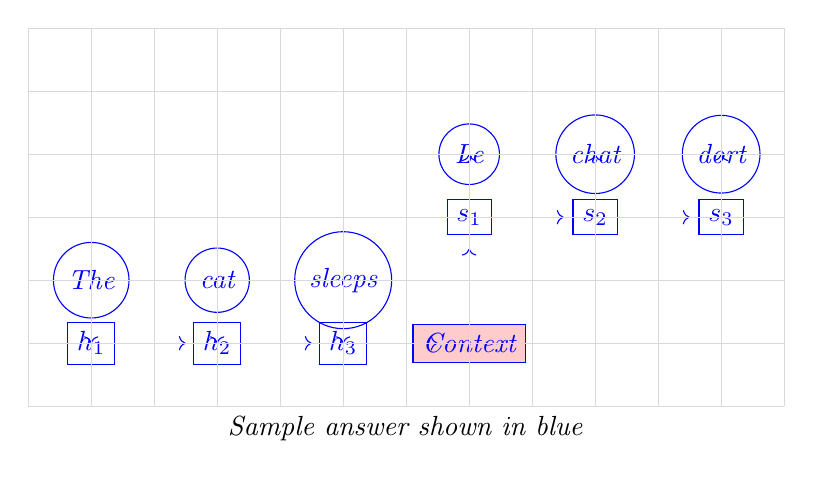
\begin{tikzpicture}[scale=0.8]
    % Sample answer overlay
    \answer{
    \node[draw, circle] at (1,2) {The};
    \node[draw, circle] at (3,2) {cat};
    \node[draw, circle] at (5,2) {sleeps};
    \draw[->] (1,1.5) -- (1,1);
    \draw[->] (3,1.5) -- (3,1);
    \draw[->] (5,1.5) -- (5,1);
    \node[draw, rectangle] at (1,1) {$h_1$};
    \node[draw, rectangle] at (3,1) {$h_2$};
    \node[draw, rectangle] at (5,1) {$h_3$};
    \draw[->] (1.5,1) -- (2.5,1);
    \draw[->] (3.5,1) -- (4.5,1);
    \node[draw, rectangle, fill=red!20] at (7,1) {Context};
    \draw[->] (5.5,1) -- (6.5,1);
    % Decoder
    \node[draw, rectangle] at (7,3) {$s_1$};
    \node[draw, rectangle] at (9,3) {$s_2$};
    \node[draw, rectangle] at (11,3) {$s_3$};
    \draw[->] (7.5,3) -- (8.5,3);
    \draw[->] (9.5,3) -- (10.5,3);
    \draw[->] (7,1.5) -- (7,2.5);
    \draw[->] (7,3.5) -- (7,4);
    \draw[->] (9,3.5) -- (9,4);
    \draw[->] (11,3.5) -- (11,4);
    \node[draw, circle] at (7,4) {Le};
    \node[draw, circle] at (9,4) {chat};
    \node[draw, circle] at (11,4) {dort};
    }
    
    % Grid for drawing
    \draw[gray!30] (0,0) grid (12,6);
    \node[below] at (6,0) {\textit{Sample answer shown in blue}};
\end{tikzpicture}
\end{center}

\teaching{Accept any reasonable architectural diagram. Key elements: encoder RNNs, context vector bottleneck, decoder RNNs, variable-length output. Students often forget the context vector or don't show the information flow clearly.}

\textbf{Question 2:} Complete the mathematical description:

\begin{itemize}
    \item Encoder equations: $h_t = $ \answer{LSTM($h_{t-1}$, $x_t$) or RNN($h_{t-1}$, $x_t$)}
    \item Context vector: $c = $ \answer{$h_T$ (final encoder state) or some function of all encoder states}
    \item Decoder equations: $s_t = $ \answer{LSTM($s_{t-1}$, $y_{t-1}$, $c$) - context influences decoder}
    \item Output probability: $P(y_t | \ldots) = $ \answer{softmax($W_s s_t + b$) or similar linear transformation}
\end{itemize}

\teaching{Don't require exact notation. Look for understanding that encoder processes input sequentially, context captures information, decoder generates output conditioned on context.}

\textbf{Question 3:} Why is the context vector a "bottleneck"?

\answer{The context vector has fixed size (e.g., 256 dimensions) regardless of input length. All information from a variable-length input sequence must be compressed into this fixed-size vector, causing information loss for long sequences. This is why translation quality degrades with sentence length in vanilla seq2seq models.}

\textbf{Question 4:} If your encoder has 128 hidden units and processes a 20-word sentence, what is the size of:
\begin{itemize}
    \item Context vector: \answer{128} dimensions
    \item Total encoder information: \answer{2560 (20 × 128)} dimensions  
    \item Information compression ratio: \answer{20:1 or 95\% compression}
\end{itemize}

\teaching{This calculation helps students understand the severity of the bottleneck problem. 95\% information loss is dramatic!}
\end{exercise}

\subsection*{A3: Attention Mechanism Deep Dive (8 minutes)}

\begin{exercise}[Attention Mathematics and Intuition]
\textbf{Question 1:} Complete the attention mechanism steps:

Step 1: Compute alignment scores: $e_{t,i} = $ \answer{align($s_{t-1}$, $h_i$) - similarity between decoder state and encoder state}

Step 2: Normalize with softmax: $\alpha_{t,i} = $ \answer{$\frac{\exp(e_{t,i})}{\sum_{j=1}^T \exp(e_{t,j})}$ - attention weights sum to 1}

Step 3: Compute context vector: $c_t = $ \answer{$\sum_{i=1}^T \alpha_{t,i} h_i$ - weighted combination of all encoder states}

\textbf{Question 2:} Given these simplified encoder states and decoder state:
\begin{itemize}
    \item $h_1 = [0.5, 0.2]$ (word: "The")
    \item $h_2 = [0.8, 0.1]$ (word: "cat") 
    \item $h_3 = [0.3, 0.7]$ (word: "sleeps")
    \item $s_t = [0.7, 0.3]$ (generating French word)
\end{itemize}

Calculate dot-product attention weights:
\begin{itemize}
    \item $e_{t,1} = h_1 \cdot s_t = $ \answer{0.5×0.7 + 0.2×0.3 = 0.35 + 0.06 = 0.41}
    \item $e_{t,2} = h_2 \cdot s_t = $ \answer{0.8×0.7 + 0.1×0.3 = 0.56 + 0.03 = 0.59}  
    \item $e_{t,3} = h_3 \cdot s_t = $ \answer{0.3×0.7 + 0.7×0.3 = 0.21 + 0.21 = 0.42}
\end{itemize}

Which word gets highest attention? \answer{"cat" ($h_2$) with score 0.59}

\teaching{Walk through the calculation step by step. After softmax, the weights would be approximately [0.27, 0.42, 0.31], so "cat" gets highest attention.}

\textbf{Question 3:} Attention visualization interpretation. If you see this attention pattern:

\begin{center}
\begin{tabular}{|l|c|c|c|c|}
\hline
\textbf{French} & \textbf{The} & \textbf{black} & \textbf{cat} & \textbf{sleeps} \\
\hline
Le & 0.8 & 0.1 & 0.1 & 0.0 \\
\hline
chat & 0.1 & 0.1 & 0.8 & 0.0 \\
\hline
noir & 0.0 & 0.9 & 0.1 & 0.0 \\
\hline
dort & 0.0 & 0.0 & 0.1 & 0.9 \\
\hline
\end{tabular}
\end{center}

What pattern do you observe? \answer{Nearly diagonal alignment - each French word attends strongly to its corresponding English word. This shows the model learned word-to-word correspondence.}

Why is this good for translation? \answer{It shows the model is learning meaningful alignments between source and target languages, rather than just using averaged information. Each output word can focus on the most relevant input words.}

\teaching{This is an idealized attention pattern. Real patterns are usually noisier but should show some meaningful structure.}
\end{exercise}

\subsection*{A4: Beam Search Strategy (4 minutes)}

\begin{exercise}[Search and Generation]
\textbf{Question 1:} Why can't we just use greedy search (always pick highest probability word)?

\answer{Greedy search can get stuck in locally optimal but globally suboptimal paths. Early high-probability words might lead to poor overall sequences. For example, starting with "The" might be locally optimal but "A" could lead to a better overall translation. Beam search explores multiple promising paths simultaneously.}

\textbf{Question 2:} Complete this beam search example (beam size = 2):

Starting with "START", expand to first word:
\begin{itemize}
    \item P("Le" | START) = 0.6
    \item P("Un" | START) = 0.3
    \item P("La" | START) = 0.1
\end{itemize}

Keep top 2: \answer{"Le"} and \answer{"Un"}

Expand "Le" to second word:
\begin{itemize}
    \item P("chat" | Le) = 0.8 → Total: \answer{0.6 × 0.8 = 0.48}
    \item P("chien" | Le) = 0.2 → Total: \answer{0.6 × 0.2 = 0.12}
\end{itemize}

Expand "Un" to second word:
\begin{itemize}
    \item P("chat" | Un) = 0.7 → Total: \answer{0.3 × 0.7 = 0.21}
    \item P("chien" | Un) = 0.3 → Total: \answer{0.3 × 0.3 = 0.09}
\end{itemize}

Final top 2 sequences: \answer{"Le chat" (0.48)} and \answer{"Un chat" (0.21)}

\teaching{Make sure students understand that we keep the globally best paths, not just the best extensions of each current path.}

\textbf{Question 3:} What happens to beam search quality vs. beam size?

Beam size 1: \answer{Equivalent to greedy search; fast but potentially poor quality}

Beam size 100: \answer{High quality but computationally expensive; may overfit to training patterns}

Optimal beam size (typical): \answer{4-8 for translation tasks; balances quality and speed}

\teaching{Emphasize the trade-off. In practice, beam size depends on the application and computational constraints.}
\end{exercise}

\newpage

\section*{Part B: Implementation and Code Understanding \hfill (15 minutes)}

\teaching{Part B tests practical understanding. Students should be able to read and debug code even if they can't write it from scratch.}

\subsection*{B1: Code Analysis (8 minutes)}

\begin{exercise}[PyTorch Implementation]
\textbf{Question 1:} Analyze this encoder code. Fill in the missing dimensions:

\begin{verbatim}
class Seq2SeqEncoder(nn.Module):
    def __init__(self, vocab_size=5000, embed_size=128, hidden_size=256):
        self.embedding = nn.Embedding(vocab_size, embed_size)
        self.lstm = nn.LSTM(embed_size, hidden_size, batch_first=True)
    
    def forward(self, x):  # x shape: [batch_size, seq_len]
        embedded = self.embedding(x)  # shape: [______, ______, ______]
        output, (h_n, c_n) = self.lstm(embedded)
        return h_n, c_n  # shapes: [______, ______], [______, ______]
\end{verbatim}

Fill in the shapes:
\begin{itemize}
    \item embedded shape: [\answer{batch\_size}, \answer{seq\_len}, \answer{128}]
    \item h\_n shape: [\answer{1}, \answer{256}] \answer{(assuming 1 layer, batch\_size implicit)}
    \item c\_n shape: [\answer{1}, \answer{256}] \answer{(same as h\_n for LSTM)}
\end{itemize}

\teaching{Shape understanding is crucial for debugging. Students often forget that LSTM returns states with layer dimension first.}

\textbf{Question 2:} What's wrong with this attention implementation?

\begin{verbatim}
def attention(decoder_hidden, encoder_outputs):
    scores = torch.matmul(decoder_hidden, encoder_outputs.T)
    weights = F.softmax(scores, dim=1)
    context = torch.sum(weights * encoder_outputs, dim=1)
    return context
\end{verbatim}

Problem: \answer{Dimension mismatch. decoder\_hidden is likely [batch, hidden] and encoder\_outputs is [batch, seq\_len, hidden]. The transpose and matrix multiplication don't align properly.}

Fix: \answer{Use torch.bmm for batch matrix multiplication or expand decoder\_hidden to match encoder\_outputs dimensions, or use Einstein summation: torch.einsum('bh,bsh->bs', decoder\_hidden, encoder\_outputs)}

\textbf{Question 3:} Complete this beam search pseudocode:

\begin{verbatim}
def beam_search(model, input_seq, beam_size=4, max_length=20):
    beams = [{"sequence": [START_TOKEN], "score": 0.0}]
    
    for step in range(max_length):
        candidates = []
        for beam in beams:
            if beam["sequence"][-1] == END_TOKEN:
                candidates.append(beam)
                continue
            
            # Get next word probabilities
            probs = model.predict_next(beam["sequence"])
            
            # Expand beam
            for word, prob in probs.top_k(beam_size):
                new_score = ___________________
                new_sequence = ______________
                candidates.append({"sequence": new_sequence, "score": new_score})
        
        # Keep top beam_size candidates
        beams = sorted(candidates, key=lambda x: x["score"])[:______]
    
    return beams[0]["sequence"]
\end{verbatim}

Fill in the blanks:
\begin{itemize}
    \item new\_score = \answer{beam["score"] + log(prob)} \answer{(or beam["score"] * prob for product)}
    \item new\_sequence = \answer{beam["sequence"] + [word]}
    \item Keep top: \answer{beam\_size}
\end{itemize}

\teaching{Emphasize log probabilities to avoid numerical underflow. Students often forget that we want the highest scores (descending sort).}
\end{exercise}

\subsection*{B2: Training Insights (7 minutes)}

\begin{exercise}[Training Process]
\textbf{Question 1:} What is "teacher forcing" and why do we use it during training?

Definition: \answer{During training, use the true target tokens as decoder inputs instead of the model's own predictions. Feed the correct previous word even if the model predicted something else.}

Why use it: \answer{Accelerates training by providing stable gradients and prevents error accumulation during training. Allows parallel computation across the target sequence.}

What problem does it cause: \answer{Exposure bias - at inference time, the model must use its own predictions, creating a mismatch between training and testing conditions. Can lead to error accumulation during generation.}

\teaching{This is a subtle but important concept. Students often struggle with understanding why training differs from inference in seq2seq models.}

\textbf{Question 2:} Loss function analysis. Given these target and predicted sequences:

Target: ["Le", "chat", "dort", "<EOS>"]
Predicted logits for each position:
\begin{itemize}
    \item Position 1: P("Le")=0.8, P("Un")=0.15, P("La")=0.05
    \item Position 2: P("chat")=0.9, P("chien")=0.07, P("oiseau")=0.03
    \item Position 3: P("dort")=0.6, P("mange")=0.3, P("court")=0.1
    \item Position 4: P("<EOS>")=0.95, P("bien")=0.03, P("mal")=0.02
\end{itemize}

Calculate the cross-entropy loss:
\begin{itemize}
    \item Position 1 loss: $-\log(0.8) = $ \answer{0.097}
    \item Position 2 loss: $-\log(0.9) = $ \answer{0.046}
    \item Position 3 loss: $-\log(0.6) = $ \answer{0.222}
    \item Position 4 loss: $-\log(0.95) = $ \answer{0.022}
    \item Total loss: \answer{0.387 (sum of individual losses)}
\end{itemize}

\teaching{Don't require precise calculations. Look for understanding that lower probabilities give higher losses, and total loss is the sum.}

\textbf{Question 3:} Why might attention weights look random at the start of training?

\answer{At initialization, the alignment function hasn't learned meaningful relationships yet. The similarity scores between decoder and encoder states are essentially random, leading to uniform or noisy attention distributions. The model hasn't learned which source words are relevant for predicting specific target words.}

What should happen to attention weights as training progresses?

\answer{Attention should become more focused and structured. For translation, we expect somewhat diagonal patterns (source word i attends to target word j). The model learns which source positions are most relevant for each target position, leading to sharper, more interpretable attention patterns.}
\end{exercise}

\newpage

\section*{Part C: Real-World Applications \hfill (12 minutes)}

\teaching{Part C connects concepts to practical applications. Look for understanding of how seq2seq principles apply to modern systems.}

\subsection*{C1: Modern Applications Analysis (6 minutes)}

\begin{exercise}[2024 Industry Applications]
\textbf{Question 1:} Map these modern systems to seq2seq components:

\begin{center}
\begin{tabular}{|l|l|l|}
\hline
\textbf{Application} & \textbf{Input} & \textbf{Output} \\
\hline
Google Translate & \answer{Source language text} & \answer{Target language text} \\
\hline
GitHub Copilot & \answer{Code context/comments} & \answer{Generated code} \\
\hline
Email Summarization & \answer{Full email content} & \answer{Short summary} \\
\hline
Text-to-SQL & \answer{Natural language query} & \answer{SQL statement} \\
\hline
Chatbot Response & \answer{User message/context} & \answer{Bot response} \\
\hline
\end{tabular}
\end{center}

\textbf{Question 2:} Which of these would benefit most from attention mechanism?
\begin{itemize}
    \item[\checkbox] Translating short phrases (3-5 words) \answer{Less critical for short sequences}
    \item[\answer{\checkmark}] Translating technical documents (500+ words) \answer{Most benefit - long sequences suffer from bottleneck}
    \item[\checkbox] Generating code from one-line comments \answer{Moderate benefit}
    \item[\answer{\checkmark}] Summarizing research papers \answer{High benefit - long input, selective attention needed}
    \item[\checkbox] Converting speech to text \answer{Different domain, but attention helps with alignment}
\end{itemize}

Explain your top choice: \answer{Long documents suffer most from information bottleneck. Attention allows the model to focus on different parts of the document when generating different parts of the summary, rather than compressing everything into a single context vector.}

\textbf{Question 3:} Compare 2014 vs 2024 seq2seq capabilities:

\begin{center}
\begin{tabular}{|l|l|l|}
\hline
\textbf{Aspect} & \textbf{2014 (Original)} & \textbf{2024 (Modern)} \\
\hline
Max input length & \answer{~20 words practical} & \answer{1000s of tokens} \\
\hline
Translation quality & \answer{25-30 BLEU} & \answer{65+ BLEU} \\
\hline
Inference speed & \answer{Slow (sequential)} & \answer{Fast (parallel/optimized)} \\
\hline
Model size & \answer{10M parameters} & \answer{100B+ parameters} \\
\hline
Applications & \answer{Research demos} & \answer{Production systems} \\
\hline
\end{tabular}
\end{center}

\teaching{Accept reasonable estimates. The key is understanding the massive scaling in all dimensions.}
\end{exercise}

\subsection*{C2: System Design Challenge (6 minutes)}

\begin{exercise}[Building Real Systems]
\textbf{Question 1:} Design a meeting summarization system:

\textbf{Input:} 2-hour meeting transcript (5000 words)
\textbf{Output:} Key points and action items (200 words)

Your architecture:
\begin{itemize}
    \item Preprocessing: \answer{Segment into sentences, remove filler words, identify speakers, timestamp key sections}
    \item Encoder design: \answer{Hierarchical encoder - sentence-level then document-level, or transformer with positional encoding for long sequences}
    \item Attention strategy: \answer{Multi-head attention to focus on different types of content (decisions, action items, key points)}
    \item Decoder design: \answer{Structured decoder that generates specific sections (decisions, actions, participants) with appropriate formatting}
    \item Post-processing: \answer{Format into bullet points, add timestamps, validate action item assignments}
\end{itemize}

\textbf{Question 2:} Code comment to function generator:

\textbf{Input:} "Function to calculate fibonacci numbers up to n"
\textbf{Output:} Complete Python function

What challenges would this face?
\begin{enumerate}
    \item \answer{Ambiguous specifications - many ways to implement fibonacci}
    \item \answer{Variable function signatures - what parameters, return types?}
    \item \answer{Style and convention consistency - naming, formatting, documentation}
\end{enumerate}

How would attention help? \answer{Attention allows the model to focus on different parts of the comment when generating different parts of the code. For example, attending to "fibonacci" when deciding on algorithm, "up to n" when handling the parameter, etc.}

\textbf{Question 3:} Multilingual customer support system:

Requirements:
\begin{itemize}
    \item Input: Customer query in any of 10 languages
    \item Output: Response in same language as input
    \item Must handle domain-specific terminology
\end{itemize}

Design approach:
\begin{itemize}
    \item Language detection: \answer{Classifier to identify input language before processing}
    \item Translation pipeline: \answer{Translate to English, process, translate back; or use multilingual model}
    \item Response generation: \answer{Seq2seq model trained on customer service conversations with domain-specific vocabulary}
    \item Quality assurance: \answer{Confidence scoring, human review for low-confidence responses, feedback loop for continuous improvement}
\end{itemize}

\teaching{Look for practical considerations: language detection, domain adaptation, quality control, human-in-the-loop systems.}
\end{exercise}

\newpage

\section*{Part D: Critical Thinking and Extensions \hfill (8 minutes)}

\subsection*{D1: Problem Solving (4 minutes)}

\begin{warning}
Real challenges you might encounter in production:
\end{warning}

\begin{exercise}[Debugging and Optimization]
\textbf{Scenario 1:} Your seq2seq translator produces repetitive output: "The cat the cat the cat sleeps"

Possible causes:
\begin{itemize}
    \item[\checkbox] Attention weights are too uniform \answer{Possible but not the main cause}
    \item[\answer{\checkmark}] Beam search beam size too small \answer{Yes - can get stuck in repetitive loops}
    \item[\answer{\checkmark}] Training data has repetitive patterns \answer{Yes - model learns from data artifacts}
    \item[\checkbox] Learning rate too high \answer{Less likely to cause this specific pattern}
    \item[\answer{\checkmark}] Decoder getting stuck in local optima \answer{Yes - especially with greedy search}
\end{itemize}

Best solution: \answer{Use coverage mechanisms, increase beam diversity, add repetition penalties during decoding, or train with more diverse data. Also check for exposure bias from teacher forcing.}

\textbf{Scenario 2:} Translation quality drops drastically for sentences longer than 20 words.

Root cause: \answer{Information bottleneck problem - fixed-size context vector cannot capture all information from long sequences. Earlier parts of the sequence are "forgotten" by the time encoding is complete.}

Solution strategy: \answer{Implement attention mechanism to allow decoder to access all encoder states, not just the final one. This eliminates the fixed-size bottleneck and allows the model to selectively focus on relevant parts of the input.}

\textbf{Scenario 3:} Your model works great on formal text but fails on casual social media language.

Why this happens: \answer{Domain mismatch between training data (likely formal text) and test data (casual language). Different vocabulary, grammar, abbreviations, and informal expressions not seen during training.}

How to fix: \answer{Domain adaptation: fine-tune on social media data, augment training with informal text, use domain adversarial training, or preprocess to normalize informal language to formal equivalents.}

\teaching{These scenarios reflect real production challenges. Emphasize that data and domain considerations are as important as model architecture.}
\end{exercise}

\subsection*{D2: Future Connections (4 minutes)}

\begin{think}
\textbf{Connecting to Advanced Topics:}

\textbf{Question 1:} How do Transformers (next week) improve on seq2seq?

Key improvements:
\begin{enumerate}
    \item \answer{Parallelization - self-attention allows parallel processing vs sequential RNN computation}
    \item \answer{Better long-range dependencies - attention connects distant positions directly}
    \item \answer{Multiple attention heads - can attend to different types of relationships simultaneously}
\end{enumerate}

\textbf{Question 2:} Modern large language models (ChatGPT, GPT-4) use modified seq2seq principles. What's different?

Architectural changes: \answer{Transformer-based (self-attention only), decoder-only architectures for autoregressive generation, much deeper networks with residual connections}

Scale differences: \answer{Billions of parameters vs millions, trained on trillions of tokens vs millions, massive computational resources}

Training approach: \answer{Pre-training on massive general text + fine-tuning/RLHF, rather than task-specific training from scratch}

\textbf{Question 3:} Beyond text, what other sequence-to-sequence problems exist?

\begin{itemize}
    \item Audio domain: \answer{Speech-to-text, music generation, audio translation}
    \item Video domain: \answer{Video captioning, action recognition, video prediction}
    \item Scientific domain: \answer{Protein folding prediction, chemical reaction prediction, DNA sequence analysis}
    \item Creative domain: \answer{Image captioning, story generation, code documentation}
\end{itemize}

\teaching{Help students see that seq2seq is a general framework beyond just translation. Many AI problems can be framed as sequence-to-sequence tasks.}
\end{think}

\hrule
\vspace{1em}

\section*{Grading Rubric}

\begin{teachingnote}
\textbf{Point Distribution (Total: 100 points)}
\begin{itemize}
    \item Part A: 40 points (Conceptual understanding - most critical)
    \item Part B: 25 points (Implementation understanding)  
    \item Part C: 25 points (Real-world applications)
    \item Part D: 10 points (Critical thinking and connections)
\end{itemize}

\textbf{Grading Guidelines:}
\begin{itemize}
    \item Full credit: Demonstrates complete understanding with correct explanations
    \item Partial credit (75\%): Mostly correct with minor gaps or inaccuracies
    \item Half credit (50\%): Shows understanding but significant errors or omissions
    \item Minimal credit (25\%): Attempted but fundamental misunderstandings
    \item No credit (0\%): No attempt or completely incorrect
\end{itemize}

\textbf{Common Student Errors:}
\begin{itemize}
    \item Confusing encoder and decoder roles
    \item Not understanding the bottleneck problem severity
    \item Thinking attention "replaces" the context vector rather than accessing all encoder states
    \item Confusing teacher forcing with beam search
    \item Focusing on linguistic differences rather than architectural limitations
\end{itemize}

\textbf{Discussion Points for Class Review:}
\begin{itemize}
    \item Why was seq2seq such a breakthrough? (Variable length capability)
    \item How does attention solve the bottleneck? (Access to all encoder states)
    \item Connection to modern transformers (self-attention evolution)
    \item Real-world considerations (data quality, domain adaptation, computational costs)
\end{itemize}
\end{teachingnote}

\section*{Self-Assessment and Next Steps}

\begin{checkpoint}
\textbf{Check your understanding level:}
\begin{itemize}
    \item[\checkbox] I can explain why seq2seq was needed (vs fixed-length RNNs)
    \item[\checkbox] I understand the encoder-decoder architecture completely
    \item[\checkbox] I can describe the information bottleneck problem
    \item[\checkbox] I can explain how attention solves the bottleneck
    \item[\checkbox] I can implement attention mechanism from scratch
    \item[\checkbox] I understand beam search vs greedy search trade-offs
    \item[\checkbox] I can design seq2seq systems for real applications
    \item[\checkbox] I see the connection to modern transformer models
\end{itemize}

\teaching{Students checking fewer than 6 items need additional review. Consider office hours or peer tutoring.}
\end{checkpoint}

\begin{realworld}
\textbf{Industry Relevance Check:}
Rate your confidence (1-5) for these career-relevant skills:
\begin{itemize}
    \item Building translation systems: \answer{Target: 3-4 for BSc students}
    \item Designing text summarization: \answer{Target: 3-4 for BSc students}
    \item Code generation tools: \answer{Target: 2-3 for BSc students}
    \item Conversational AI systems: \answer{Target: 3-4 for BSc students}
    \item Understanding modern LLM architecture: \answer{Target: 4-5 for BSc students}
\end{itemize}
\end{realworld}

\vspace{1em}

\textbf{Areas needing review:} \answer{Most commonly: attention mechanism details, beam search vs greedy trade-offs, connection to transformers}

\textbf{Most interesting discovery:} \answer{Often: how attention solves the bottleneck problem, or connection to modern AI systems they use daily}

\textbf{Connection to your projects/interests:} \answer{Look for genuine engagement - these students may benefit from research projects or advanced courses}

\hrule
\vspace{1em}

\section*{Next Steps}

\textbf{Immediate review:} Focus on areas where you scored below 3/5

\textbf{Hands-on practice:} 
\begin{itemize}
    \item Implement seq2seq from scratch in your preferred framework
    \item Try the model on a different language pair
    \item Experiment with different attention mechanisms
    \item Build a simple summarization system
\end{itemize}

\textbf{Preparation for Week 5:}
\begin{itemize}
    \item Review attention mechanism thoroughly
    \item Understand the limitations of RNN-based seq2seq
    \item Think about parallelization challenges
    \item Read "Attention Is All You Need" paper introduction
\end{itemize}

\teaching{Encourage students to implement a small seq2seq project before moving to transformers. The hands-on experience helps solidify concepts.}

\vspace{2em}
\begin{center}
\textbf{--- End of Assessment ---}\\
\vspace{0.5em}
\textit{You're now ready to understand how Transformers revolutionized this field!}
\end{center}

\end{document}